\documentclass{article}
\usepackage[utf8]{inputenc}
\usepackage[margin=0.70in]{geometry}
\usepackage{hyperref}
\usepackage{graphicx}
\usepackage{authblk}
\usepackage{subfig}

\title{Enabling GPU Support on NumS}
\author{Brian Park}
\author{Kunal Agarwal}
\author{Parth Baokar}
\affil{UC Berkeley, Computer Science 267}
\date{May 2022}

\begin{document}

\maketitle

\section*{Abstract}
NumS is a library that translates Python and NumPy to optimized distributed systems code. Originally, it was built on top of Ray and was intended for cloud computing environment. We explore how to implement a GPU backend that can be deployable on HPC systems with multi GPU configurations, such as NVIDIA V100 cluster connected with NVLink. We implement a GPU backend that uses CuPy to execute kernels on NVIDIA GPUs and evaluate the performance on multi GPU setup with Ray and NCCL.

\section{Introduction}
Nowadays, there are many parallel primitives that can be used to accelerate numerical workloads. The most popular ones by far for the CPU have been OpenMP, MPI, and UPC++. But often, CPUs do not meet the demand of compute power coming from deep learning models, often requiring petabytes/s of throughput \cite{openai}. Figure \ref{fig:openai} shows that the increase in compute power over the past decade. This is where domain specific hardware is needed, such as GPUs and TPUs to bridge the gap between compute power today's hardware provides and the growing demand from deep learning. But even then, GPUs and TPUs are often limited by the small size of high bandwidth memory to store parameters for machine learning. Due to the death of Moore's Law and end of Denard's scaling, distributed systems is often the solution to scale indefinitely. Here, we will analyze and evaluate the performance and design of NumS with single GPU and multi GPU inter-node backends to reach teraflops/s of performance.

\begin{figure}
	\centerline{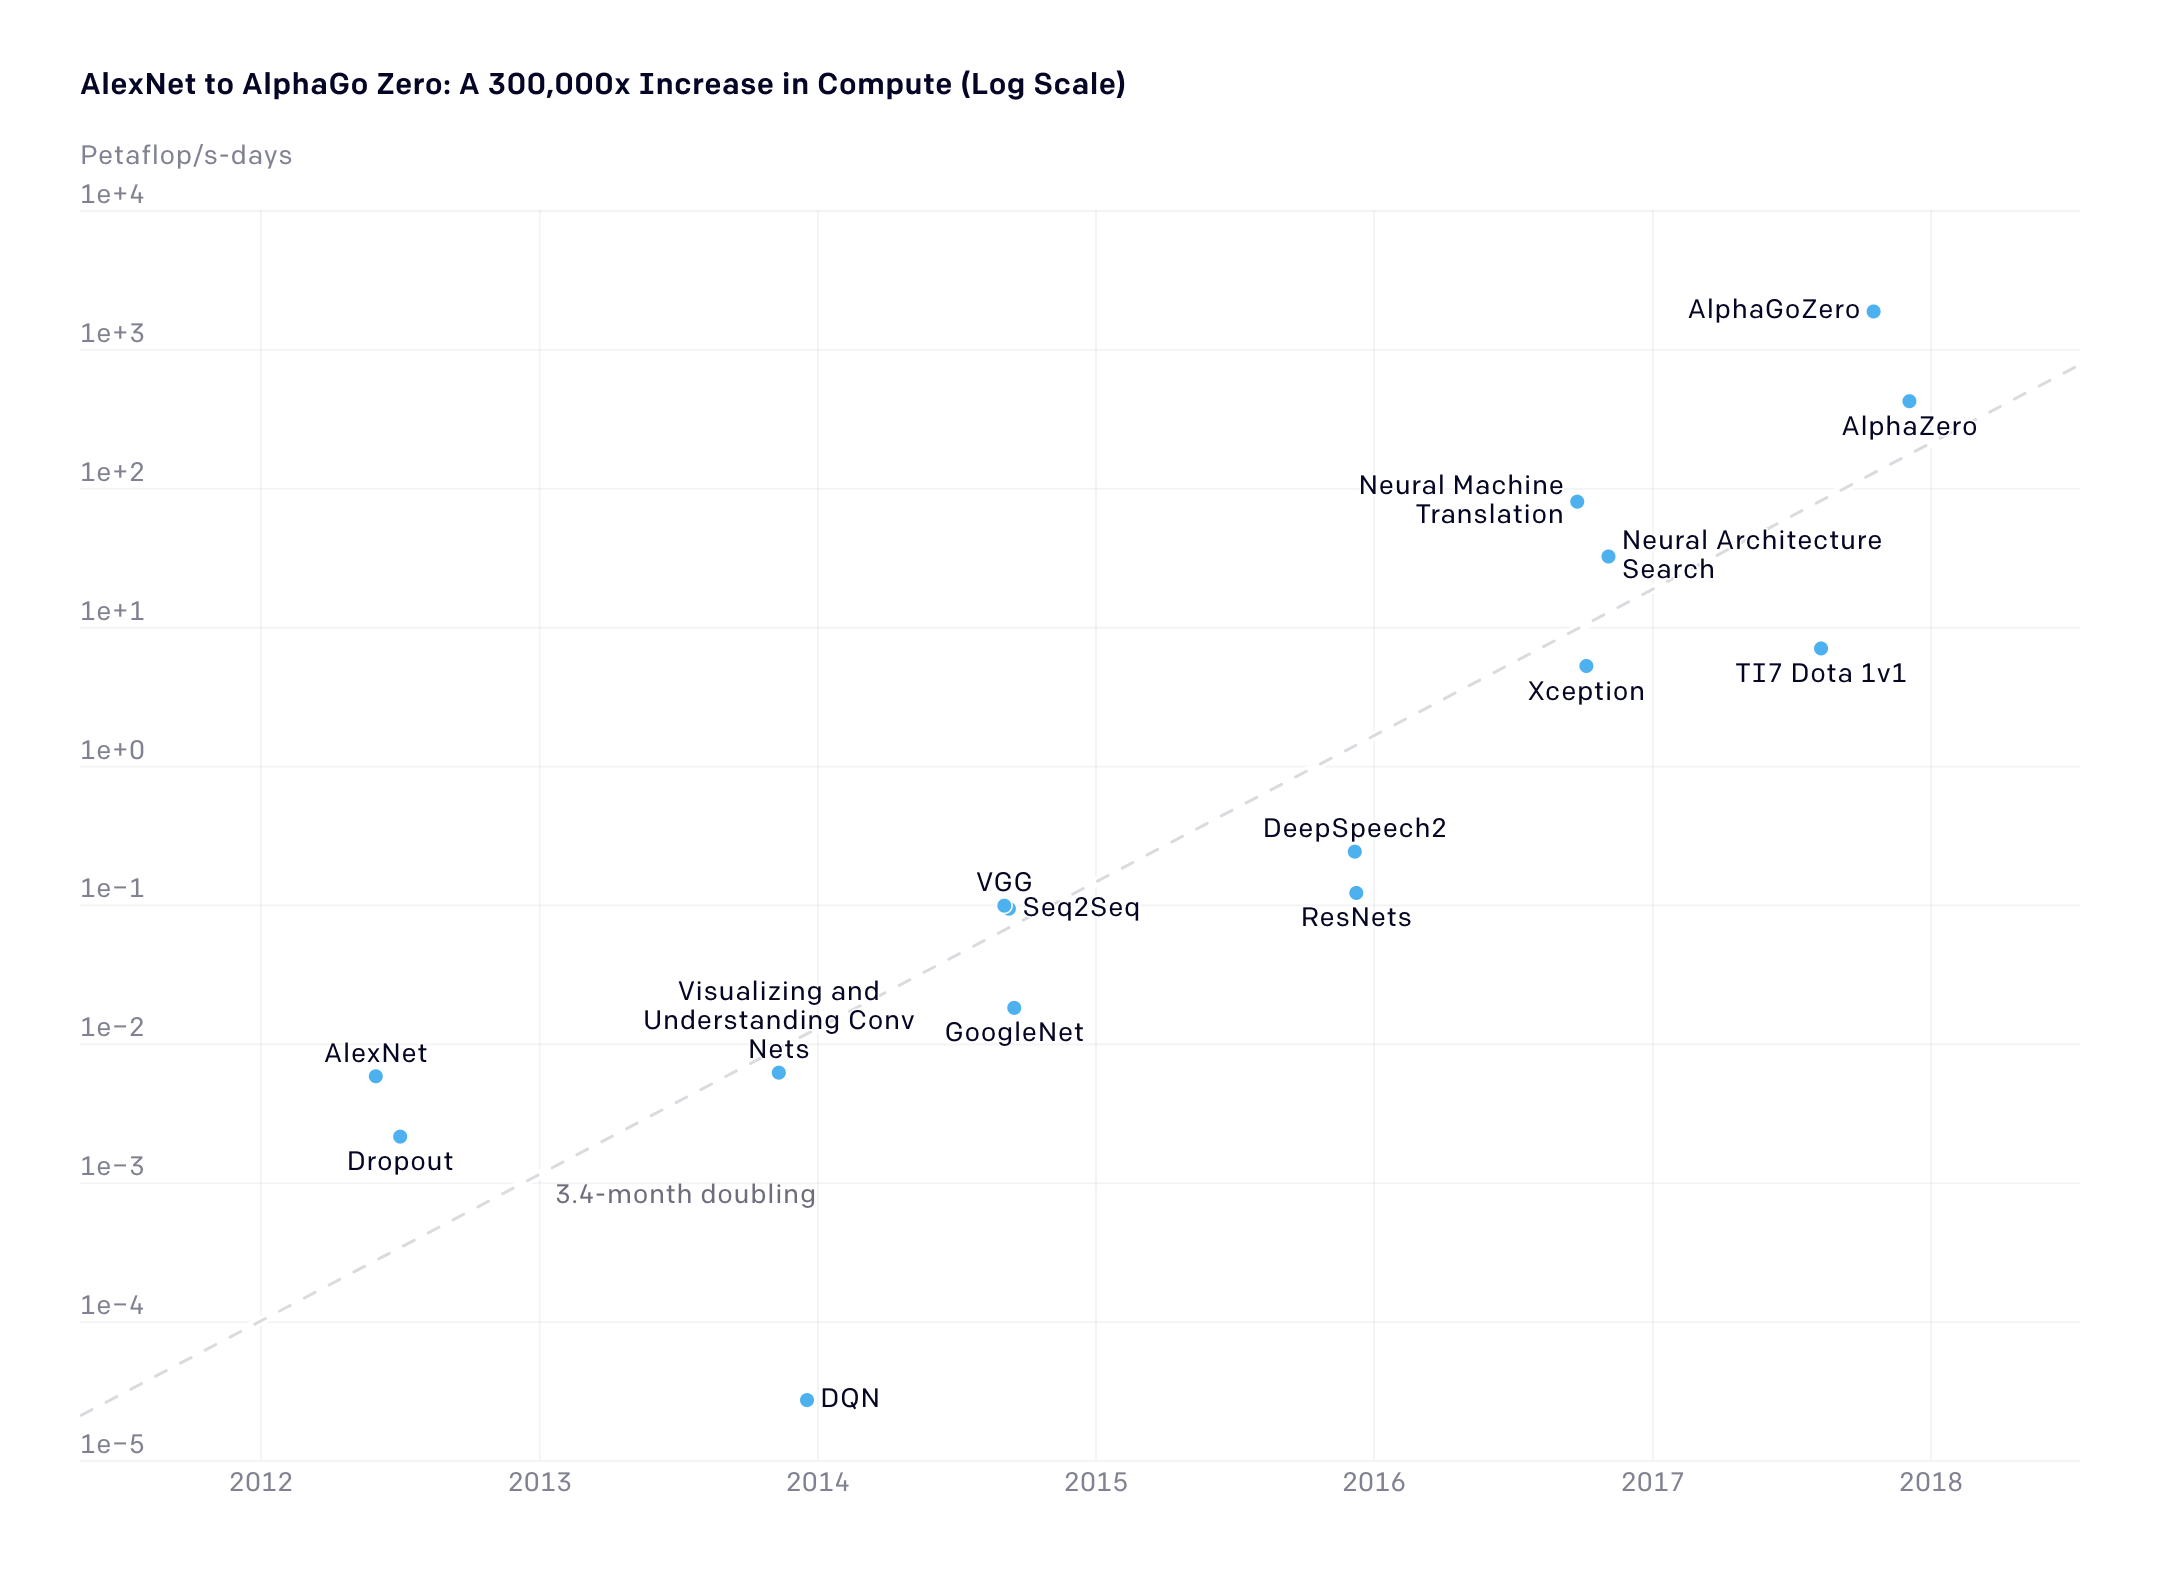
\includegraphics[width=3in]{figures/ai-and-compute-modern-log.png}}
	\caption{Compute Demands of Machine and Deep Learning Models}
	\label{fig:openai}
\end{figure}

\section{Design}
NumS by design already tries to optimize for distributed systems by providing optimal schedulers and communication avoiding algorithms. \cite{nums} We find that these same algorithms can be easily transferable when implementing a multi GPU backend.

The core backend of NumS uses NumPy for numerical computations and it has a kernel interface where computations are executed by partitions in a map-reduce style of programming. NumS has kernels written in NumPy that execute on each data partition in a SPMD style interface. For communication, an application level interface is used to coordinate data movement and scheduling between devices. Because it was originally written in Ray, the communication APIs are abstracted away from the developer using Ray's object store. The object store is an in-memory distributed object store, using futures and promises to enable task parallelism \cite{ray}. It abstracts away the communication to the developer, making writing distributed programming simple. NumS is able to be aware of array partitioning, placement, and scheduling by utilizing advanced Ray API functionality. NumS uses a data structure called BlockArray to partition the array evenly into blocks that are mapped to each CPU core. In addition to Ray, it also supports a backend for Dask and MPI, so that it could be more easily deployable on a HPC environment. Highlighted in green in Figure \ref{fig:system_arch} is the backends and interfaces implemented in this report.

\begin{figure}
	\centerline{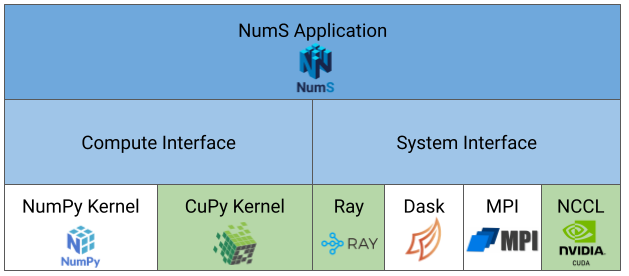
\includegraphics[width=3in]{figures/system_architecture.png}}
	\caption{System Architecture of NumS}
	\label{fig:system_arch}
\end{figure}

CuPy is a NumPy/SciPy-compatible array library for GPU-accelerated computing with Python. It can be often used as drop-in replacement for NumPy, and we use it to enable GPU support on NumS. \cite{cupy} Just like how NumPy can use optimized vendor libraries for BLAS like Intel MKL, CuPy uses NVIDIA's cuBLAS on NVIDIA GPUs while also being aware of NVIDIA hardware features such as NVIDIA Tensor Cores. Thus, CuPy serves as a viable option for NumS compared to other array libraries like Dask, Jax, or Numba. This also means that the scope of GPU support on NumS is only limited to NVIDIA GPUs with CUDA support. For BlockArray partitioning, we will map a block to a GPU, as there is no control at the CuPy API level to control thread blocks and kernel grids.

Another reason why CuPy serves as a viable option is because it also provides low level CUDA API support such as Python wrappers over the NCCL library. This allows us to write distributed code for NVIDIA GPUs using NCCL as opposed to other options such as CUDA-aware MPI. Another benefit of using NCCL is that it can be used in a single process, where it wont be a problem with Python's global interpreter lock. But it also means it will introduce latencies of function dispatch, as we observe from profiling results below.

Here, we'll explore how we implement GPU support with one GPU and extend it to two more approaches when implementing multi-GPU support with Ray and NCCL. We chose to explore Ray in order to be faithful with the already existing CPU Ray implementation of NumS.

\subsection{Serial}
We implemented the simple serial model, where NumS only uses 1 GPU. This implementation was very simple to implement as we used CuPy as our kernel interface. Properly implementing this gave us a starting point before we extended it to a multi GPU setup. Some basic synchronization primitives have to be implemented such as synchronizing GPU threads and only transferring from GPU memory to main memory when results are needed to be served to the user.

\subsection{Ray}
For implementing the multi-GPU support, we find that Ray's features to abstract away distributed code to the developer and user can be a drawback. Ray's Object Store was meant to be a way to provide a fault tolerant distributed memory model. \cite{ray} This causes a huge latency when doing computations on the GPUs, as Ray enabled functions with CuPy would forcefully route data transfers from CPU to GPU and back from GPU to CPU. This is because Ray exclusively models the Object Store as main memory, and does not include GPU memory in the model. Because low level control is abstracted away, such as explicitly transferring data between nodes or scheduling operations, implementing a high performance GPU backend becomes more of a challenge to implement. Ray was also meant to accelerate task parallelism. Although NumS is successfully able to use Ray features to enable data parallelism computations, Ray's features for data parallelism with GPU is not well supported yet. Ray also provides a collective communication library that can use NCCL to bypass data transfers to the object store. It seems to be successful in Alpa, where they use stateful Ray actor implementations \cite{alpa}. But the design of NumS was built on top of Ray remote functions which are stateless. Trying to incorporate an actor implementation would require a redesign of the NumS system architecture.

\subsection{NCCL}
With NCCL communication, there are some disadvantages over Ray that NCCL does not supply, such as not being fault tolerant and being susceptible to a deadlock. If a device goes offline in the middle of communication call, this is where NCCL fails to continue, while a Ray implementation can continue on. But since the focus of this implementation was to make NumS deployable under a HPC environment, NCCL served as a better choice in this use case, as these problems are more susceptible in cloud computing.

When using NCCL, we also had to use multiple CUDA streams to enable concurrency. Naively running code on multiple GPUs will all sync up to the null thread and serialize the timeline, disabling concurrency. For communication under NCCL, we used simple \verb|send|/\verb|recv| calls.

For scalability, we find that we cannot scale easily to more than 4 GPUs. Invalid memory accesses would happen and it could be due to data not being available yet due to a higher latency between send and receive calls. Figure \ref{fig:nvlink} shows the NVLink mappings and we see longer traversal of communication if a GPU on the left side wants to communicate with a GPU on the right side.

\begin{figure}
	\centerline{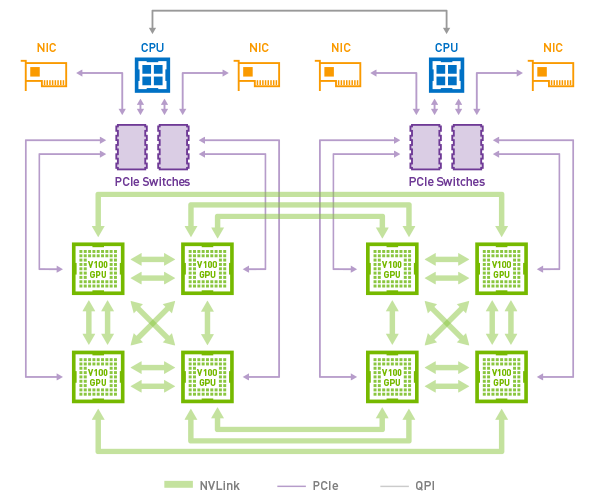
\includegraphics[width=5in]{figures/nvlink.png}}
	\caption{NVLink Topology in DGX-2 System}
	\label{fig:nvlink}
\end{figure}

\section{Evaluation}
This is one of the first applications where NumS has successfully run on a HPC machine environment. Ray was not intended to run on HPC systems, as mentioned in a guest lecture by Stoica. \cite{ray-lecture} An attempt to benchmark on Cori's Intel KNL CPUs was made, but it's performance was unstable. Instead, we benchmarked on Bridges-2 Intel Cascade Lake CPUs and their NVIDIA V100 GPUs. We evaluate microbenchmarks of GEMM routines of varying precision and some machine learning models.

\subsection{Profiling}
We see that for elementwise operations that don't require communication, there is latency involved when trying to execute CUDA kernel calls. This may be a limitation due to Python and the latency show in Figure \ref{fig:stream} is around 3 milliseconds.

\begin{figure}
	\centerline{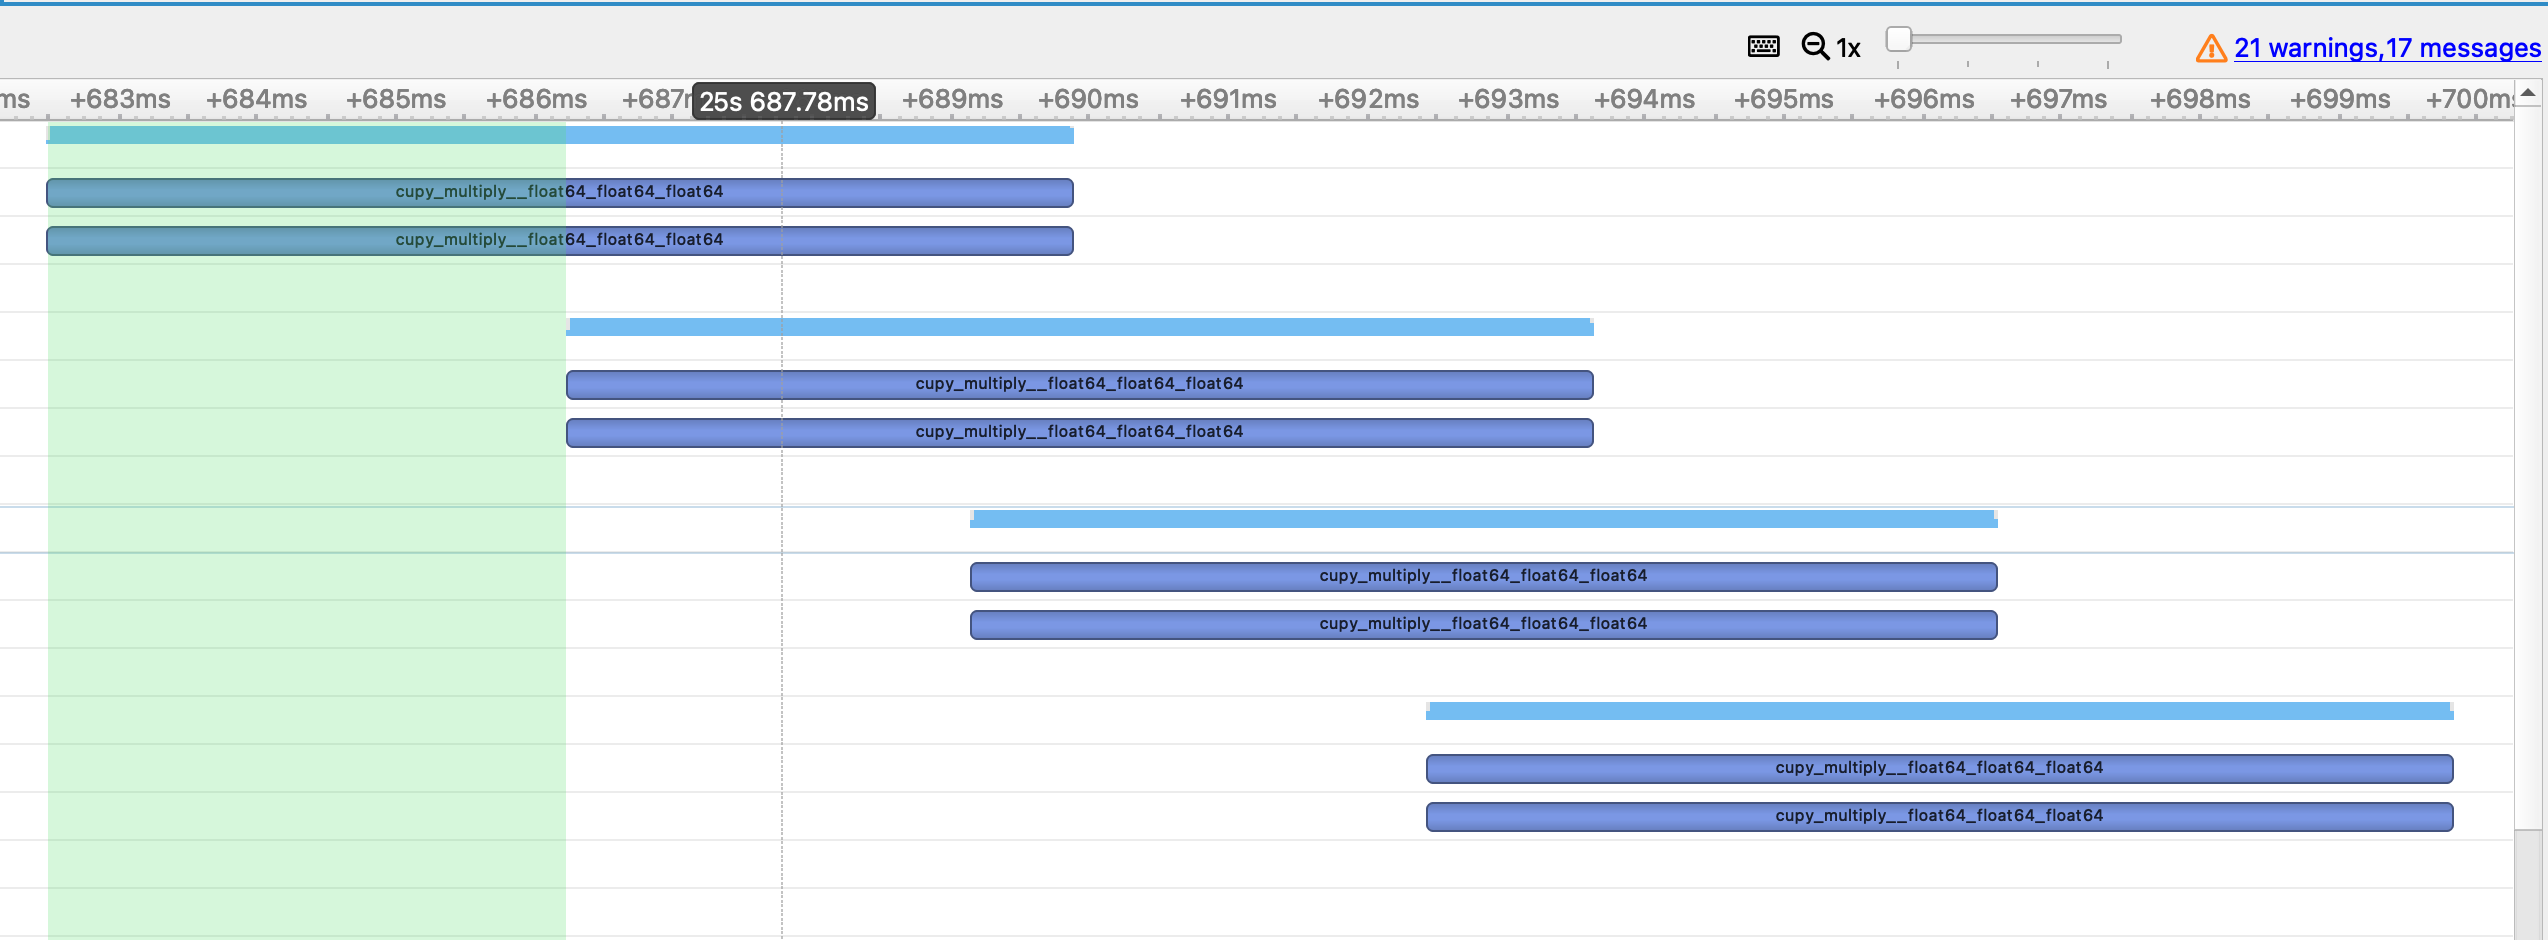
\includegraphics[width=6in]{figures/stream.png}}
	\caption{Latency of CUDA Kernel Execution}
	\label{fig:stream}
\end{figure}

For computations that used communication, we were also able to profile the NCCL communication calls. In Figure \ref{fig:nccl-dgemm}, the gray colored events are NCCL API calls, while the blue events are either DGEMM microkernel calls to cuBLAS or NCCL \verb|send|/\verb|recv|.

\begin{figure}
	\centerline{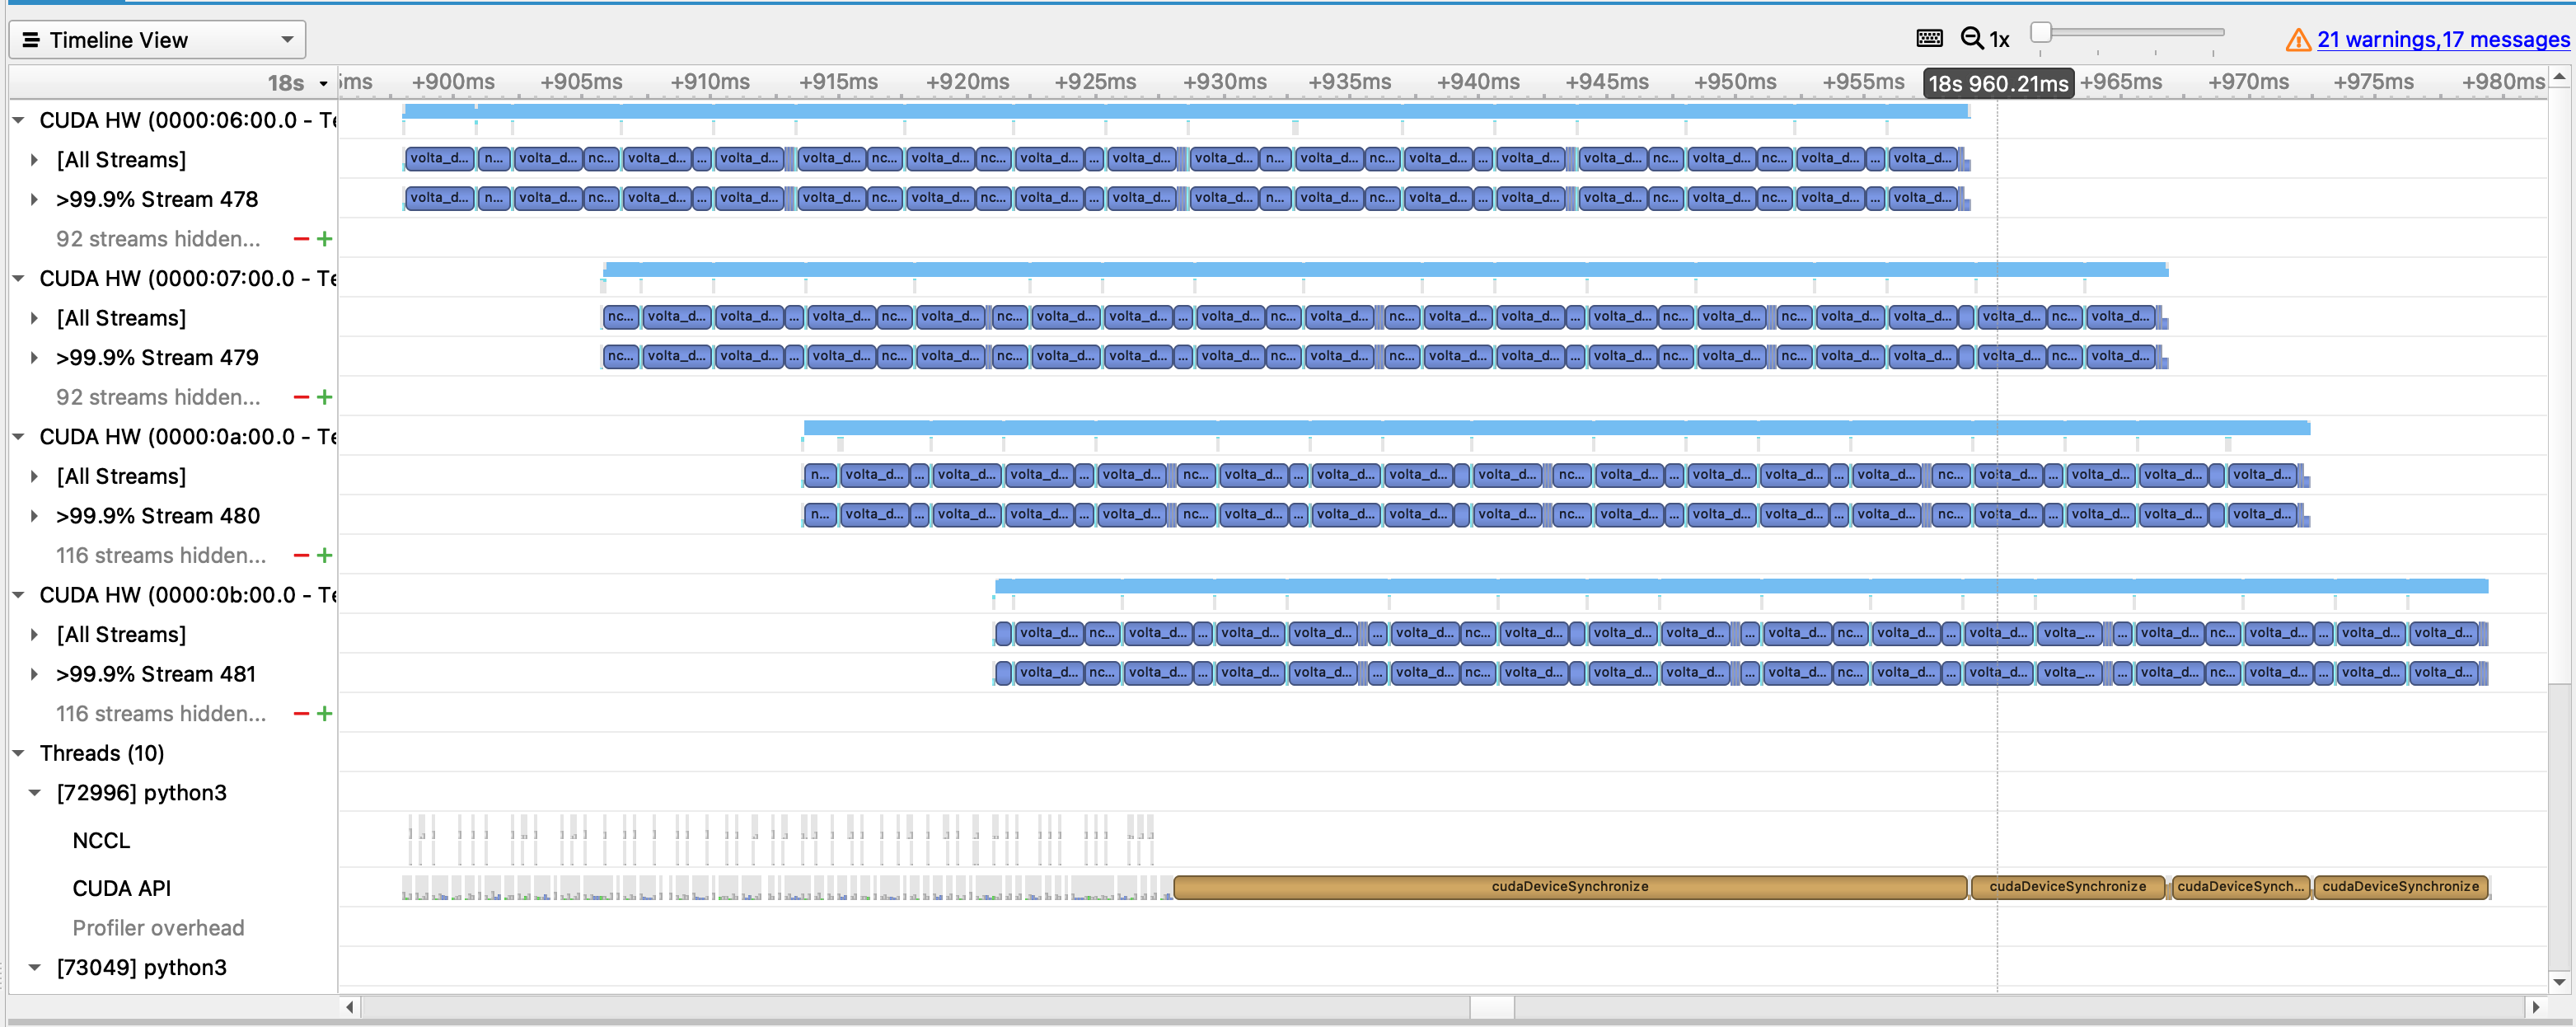
\includegraphics[width=6in]{figures/nccl-dgemm.png}}
	\caption{Multi-GPU DGEMM with NCCL Profiling}
	\label{fig:nccl-dgemm}
\end{figure}

\subsection{Benchmarks}
Benchmarking was done on Pittsburgh Supercomputing Center's Bridges-2. They have a \verb|GPU|, \verb|GPU-shared| node that uses up to 8 NVIDIA Tesla V100-32GB SXM2 GPUs and two Intel Xeon Gold 6248 “Cascade Lake” CPUs (20 cores, 2.50–3.90GHz, 27.5MB LLC, 6 memory channels) \cite{psc}. The GPUs are linked with NVLink, which provide 25 Gb/s of bandwidth. CPU benchmarks to compare the GPU backend were benchmarked against the Bridges-2 CPU node.

For each matrix multiply benchmark we seeded the random value at every iteration and generated 2 random $n \times n$ matrices to compute $C =  A \times B$. For elementwise, we did the same random seeding, but generated a size $n$ vector and did elementwise multiply. 15 trials per each size is done and the first 5 results are thrown away. This is due to CuPy initializing a CUDA context upon every first CUDA API call. Then the mean of the 10 results are taken and logged.

\subsubsection{DGEMM}
For a single GPU, William analyzes the Roofline model of V100 architecture theoretically and empirically. The theoretical peak observed for double precision floating point operations in NVIDIA V100 is 7833.6 GFLOP/s while the empirical peak is 7068.9 GFLOP/s \cite{roofline}. We observe by using CuPy's cuBLAS, it will reach near theoretical peak (94.16\%) and overachieves the empirical peak (103.91\%). We suspect that the outperformance of the empirical peak may be due to inaccuracy of timing between Python and CUDA interface that CuPy provides, or the fact that William used \verb|nvprof| and there is profiling overhead collected in the empirical peak. Figure \ref{fig:dgemm} shows the performance of NumS on multiple GPUs. NumS peak performance of each GPU setting maintains 89.2-99.86\% of the empirical peak and 80.84-90.50\% of the theoretical peak. The efficiency decreases as we increase to more GPUs, and this is likely due to communication overhead.

\begin{figure}
	\centerline{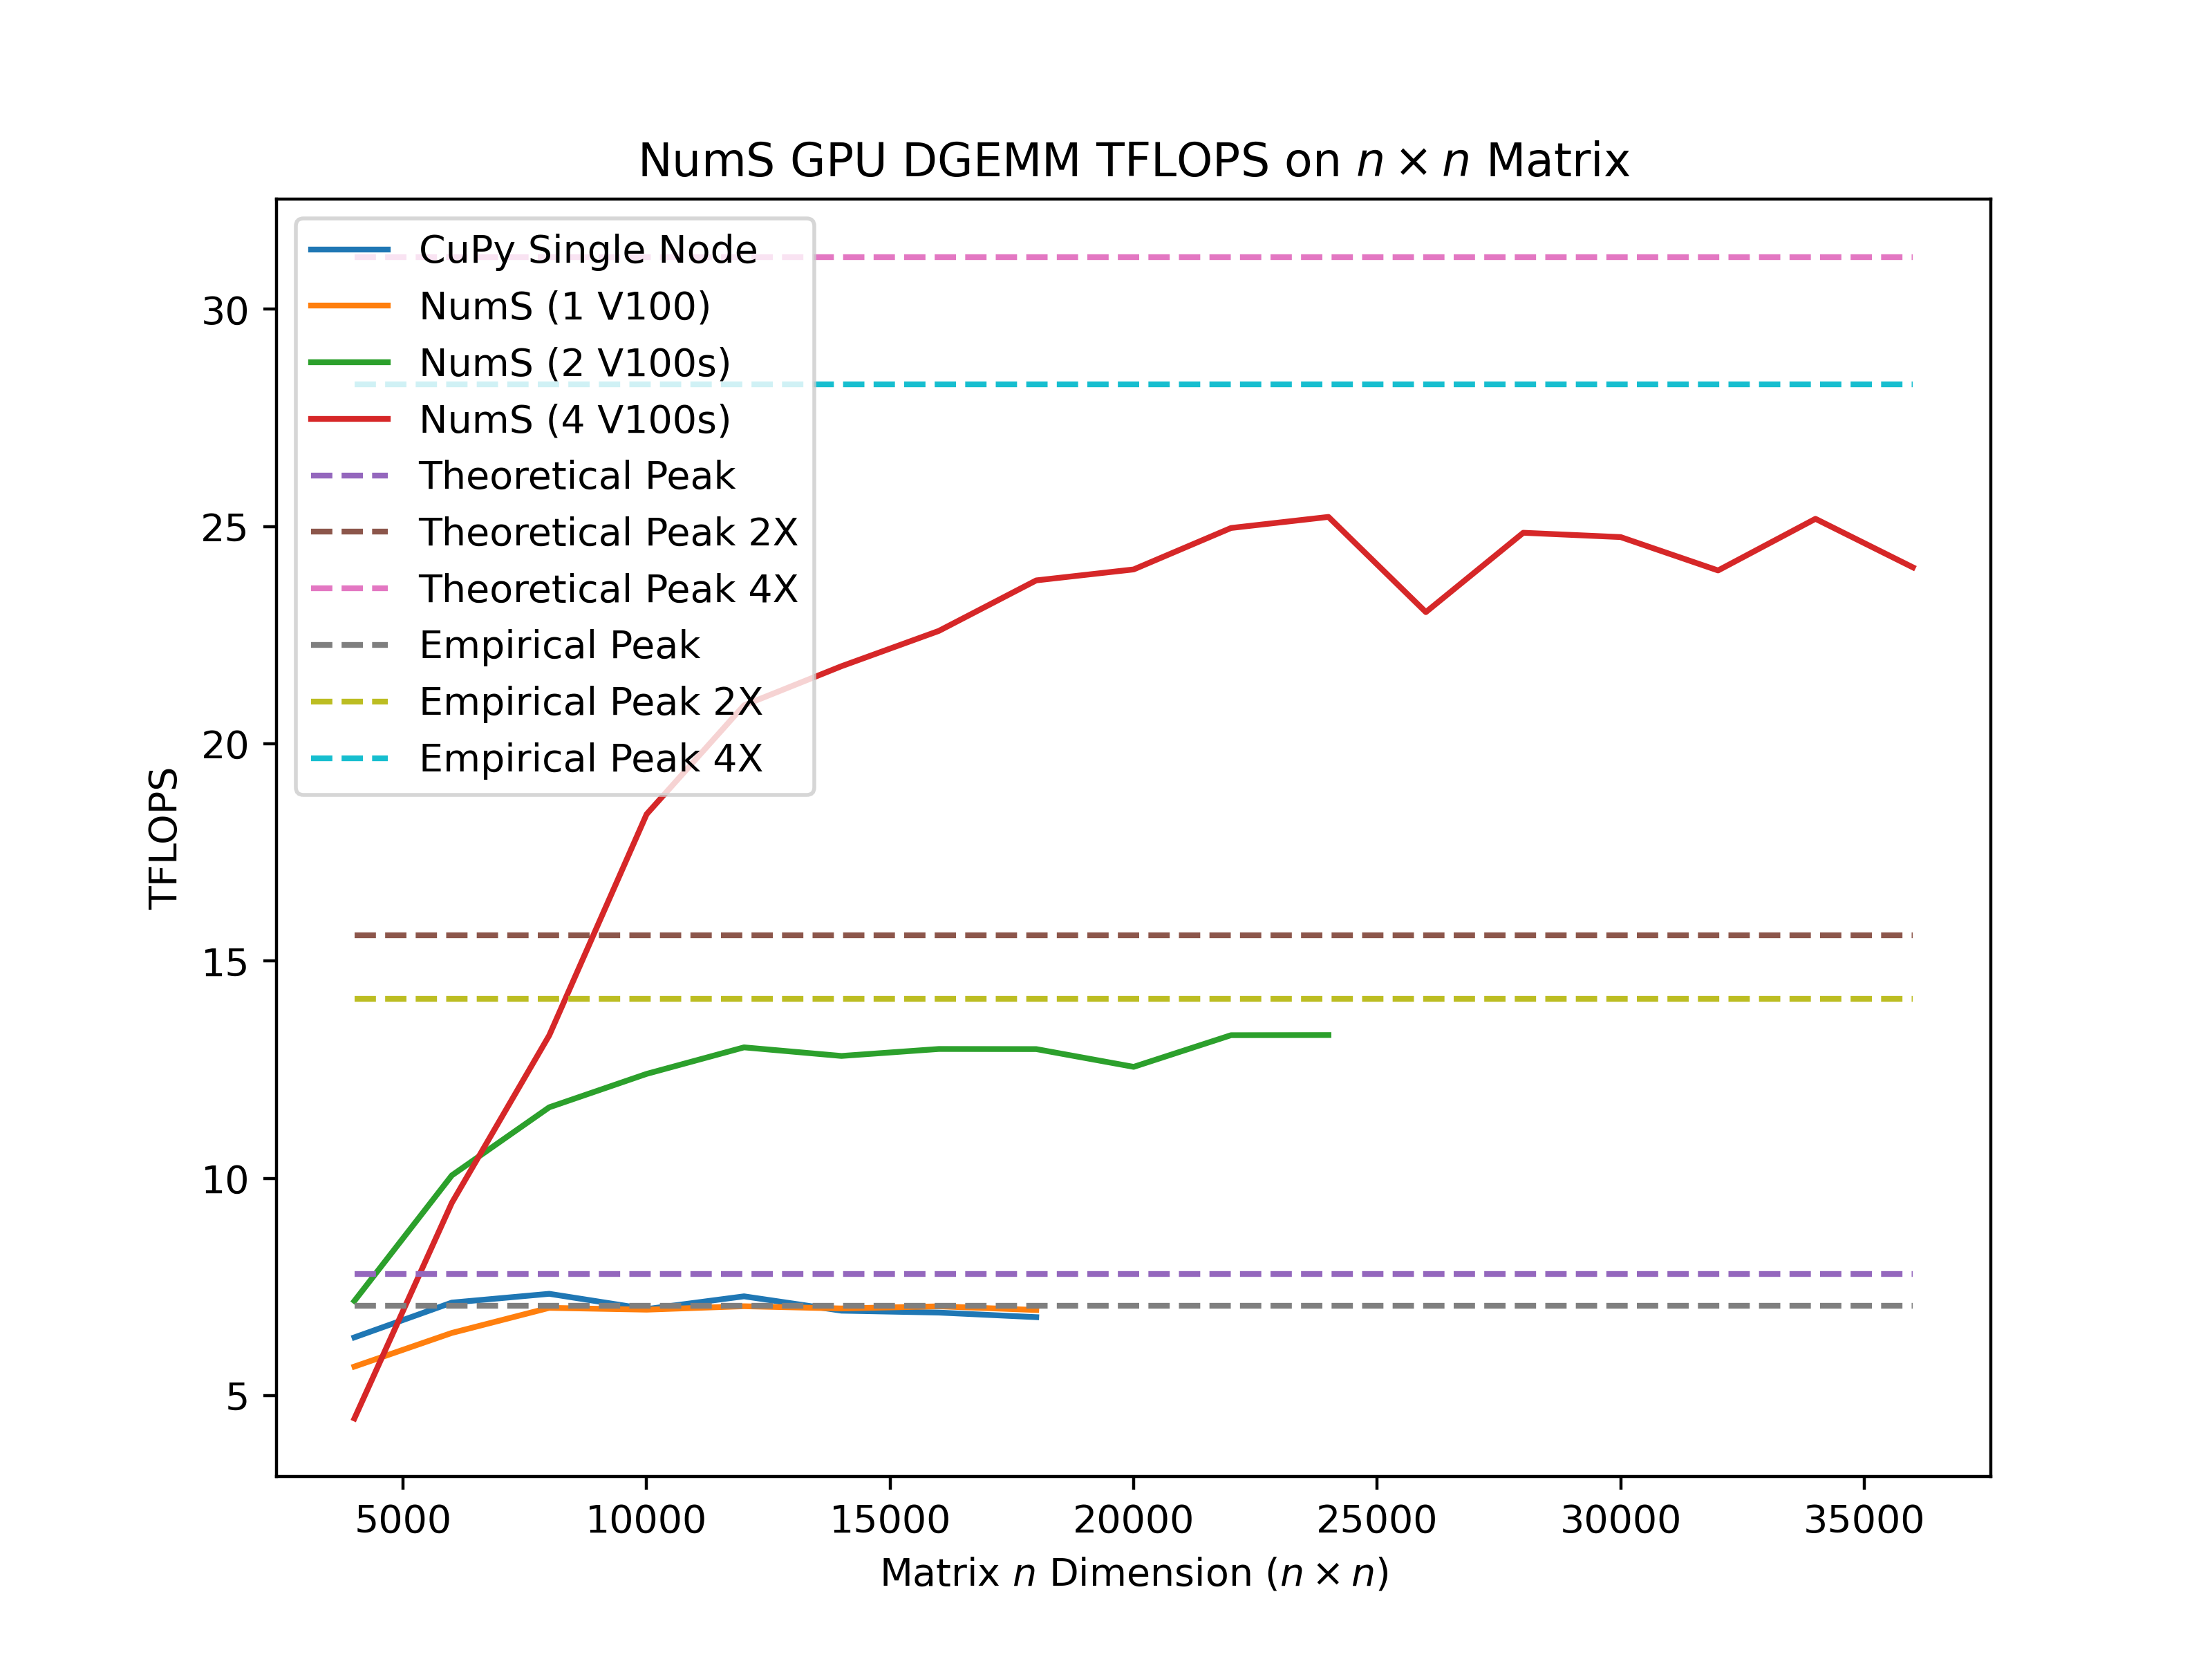
\includegraphics[width=5in]{figures/NumS_GPU_TFLOPS_DGEMM.png}}
	\caption{TeraFLOPs DGEMM Benchmark (Missing data in graph is OOM)}
	\label{fig:dgemm}
\end{figure}

\subsubsection{SGEMM}
The theoretical peak of NVIDIA V100 for single precision floating point numbers become nearly twice, 15.7 TFLOP/s. The same sizes are tested as NumS by default generates random double precision floating point numbers. We only transform matrices $A, B$ to single precision after they have been generated. Figure \ref{fig:sgemm} shows SGEMM performance on NumS up to 4 GPUs. NumS peak performance maintains 80.84-90.18\% of the theoretical peak in single precision performance. This is very similar performance from the DGEMM, and we see that the difference in precision scales well.

\begin{figure}
	\centerline{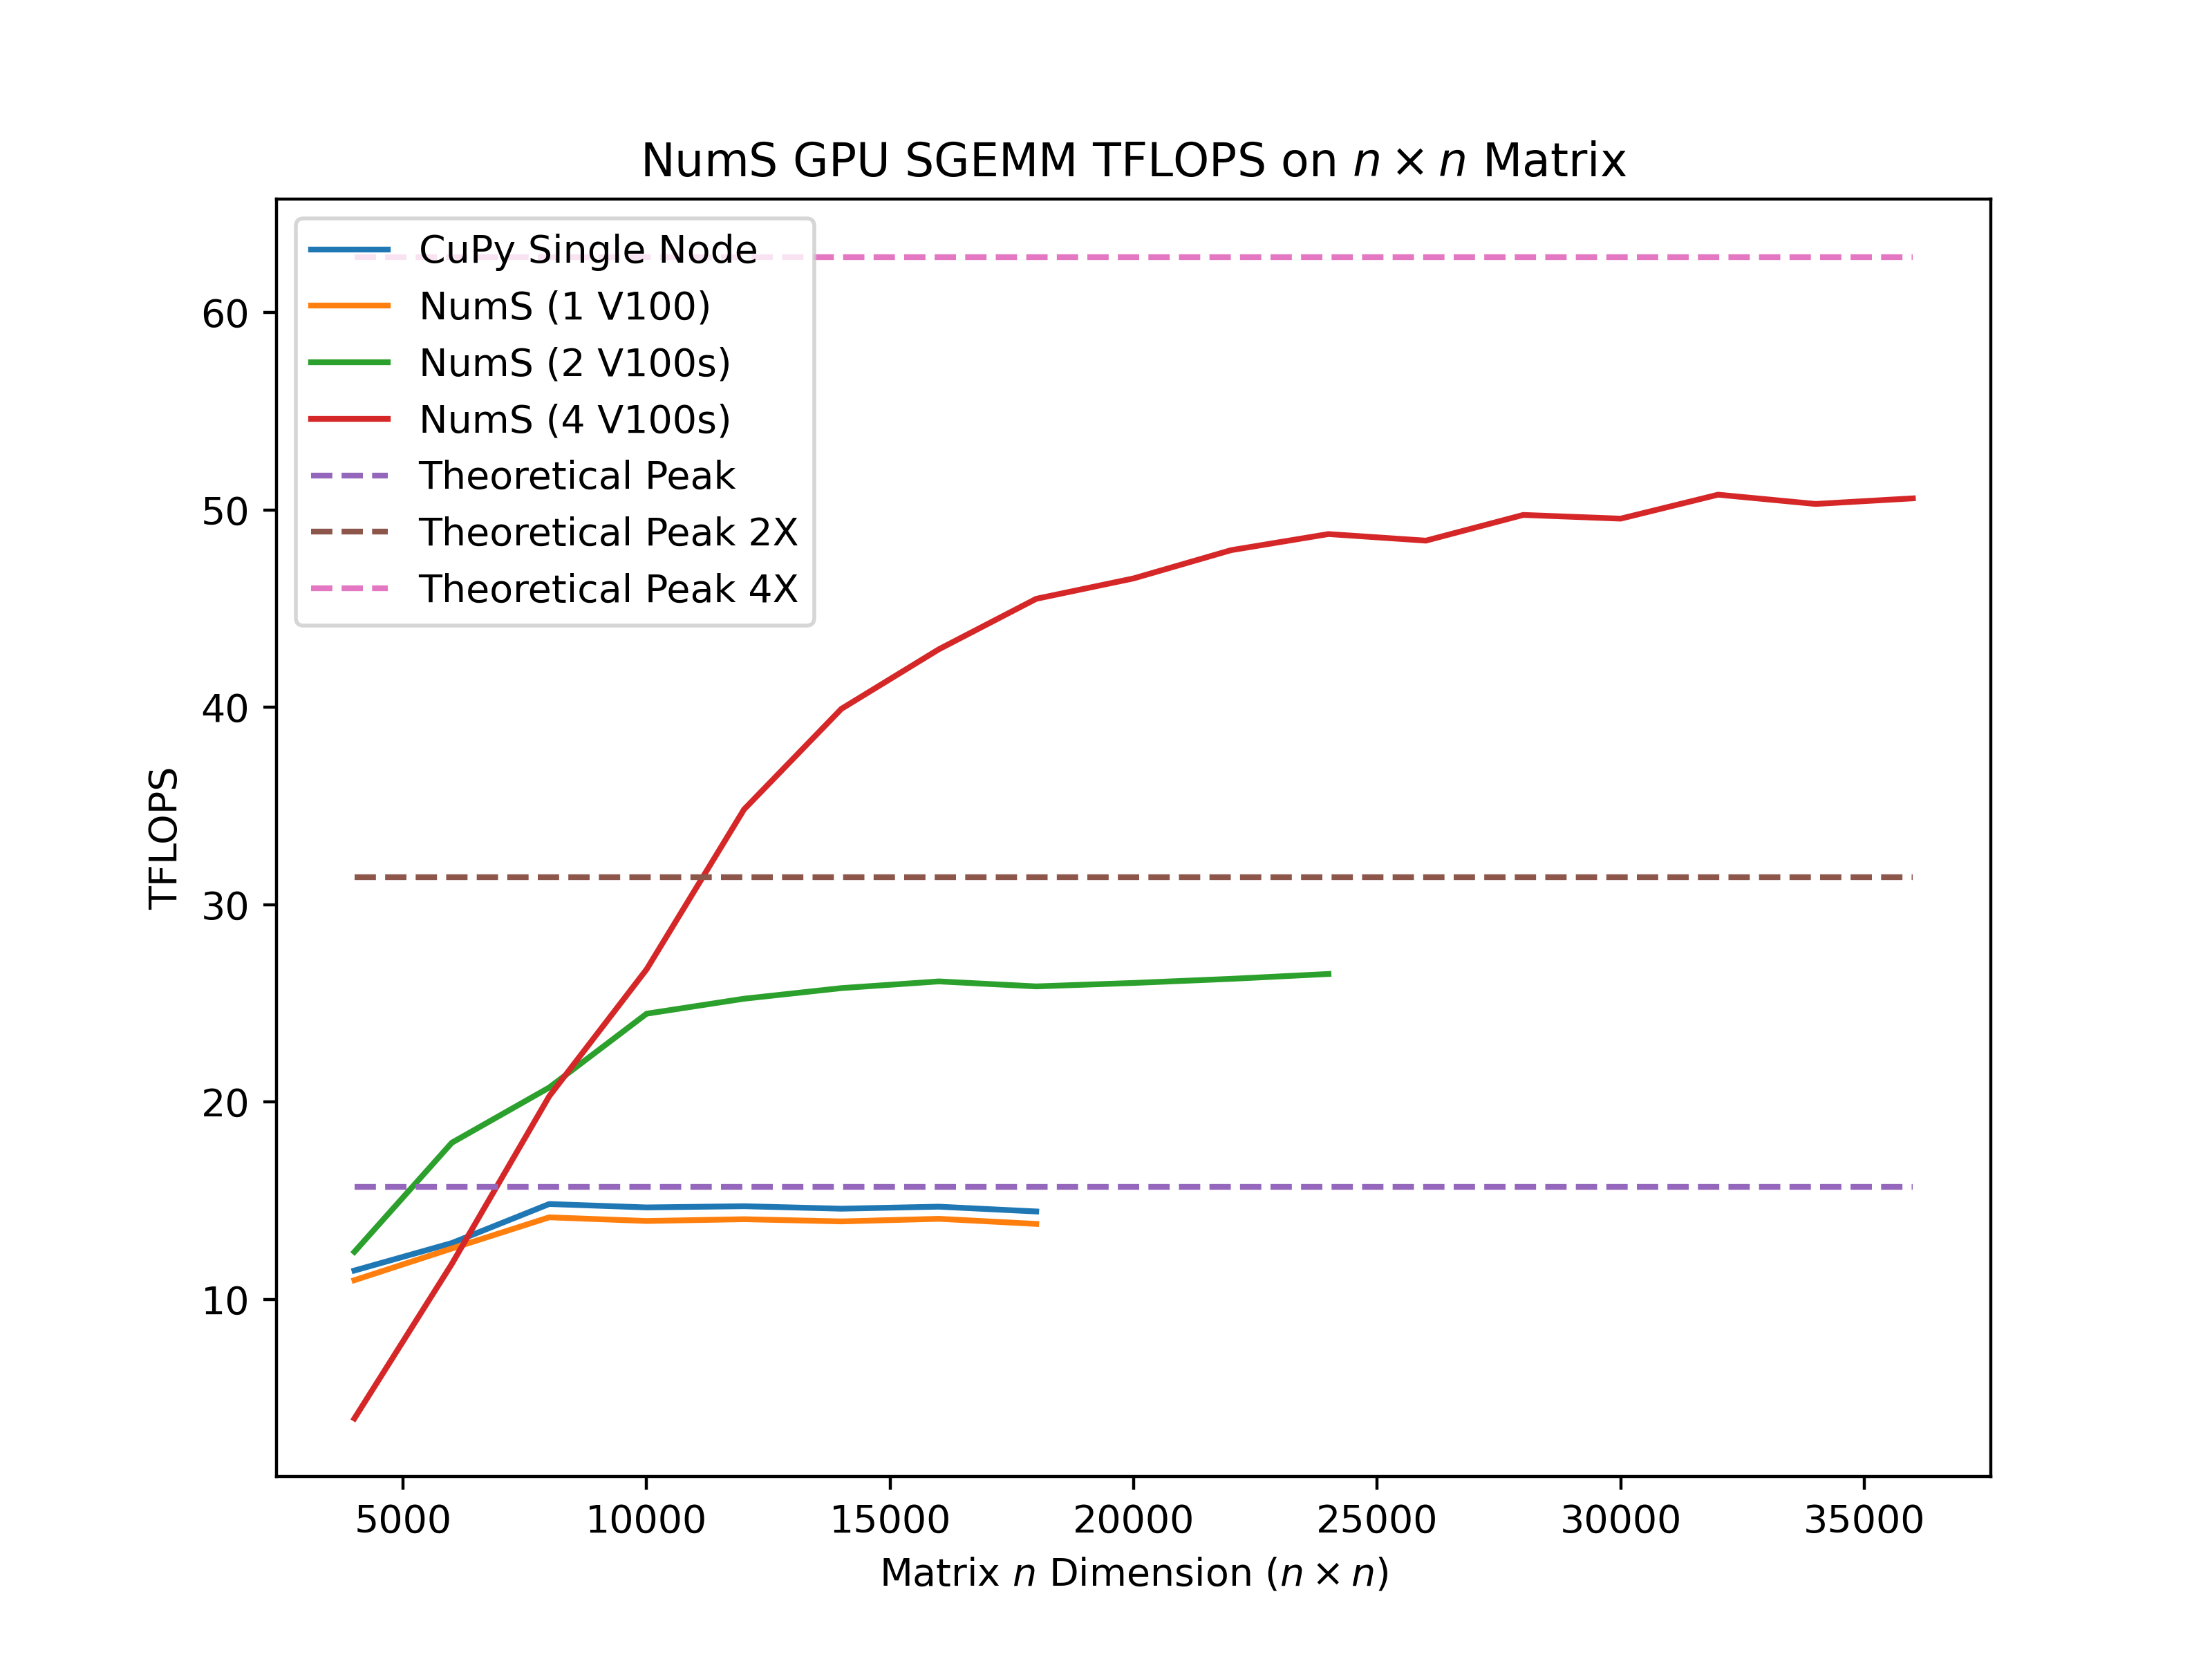
\includegraphics[width=5in]{figures/NumS_GPU_TFLOPS_SGEMM.png}}
	\caption{TeraFLOPs SGEMM Benchmark}
	\label{fig:sgemm}
\end{figure}

\subsubsection{Half Precision FP16 GEMM}
Half precision computations are useful where high precision doesn't matter and speed is important. CPU architectures and software are not well supported for these types of computations. For example, NumPy cannot compute FP16 as many Intel architectures do not support \verb|fmadd| for FP16 SIMD vectors. NVIDIA V100 architecture is able to provide Tensor Cores, which use specialized hardware accelerators and are able to hit a theoretical peak of 125 TFLOP/s.

Figure \ref{fig:fp16gemm} shows the performance of half precision GEMM on NumS up to 4 GPUs. NumS peak performance maintains between 54.78-77.44\% of the theoretical peak for Tensor Cores. Unfortunately, when scaling to more than 1 GPU, the percentage of theoretical peak goes down more quickly compared to DGEMM and SGEMM. And from the start, the theoretical peak for Tensor Core could not be reached with high efficiency. There is still more work to be done here to understand why scaling is not as efficient and the base performance is not ideal to begin with.

\begin{figure}
	\centerline{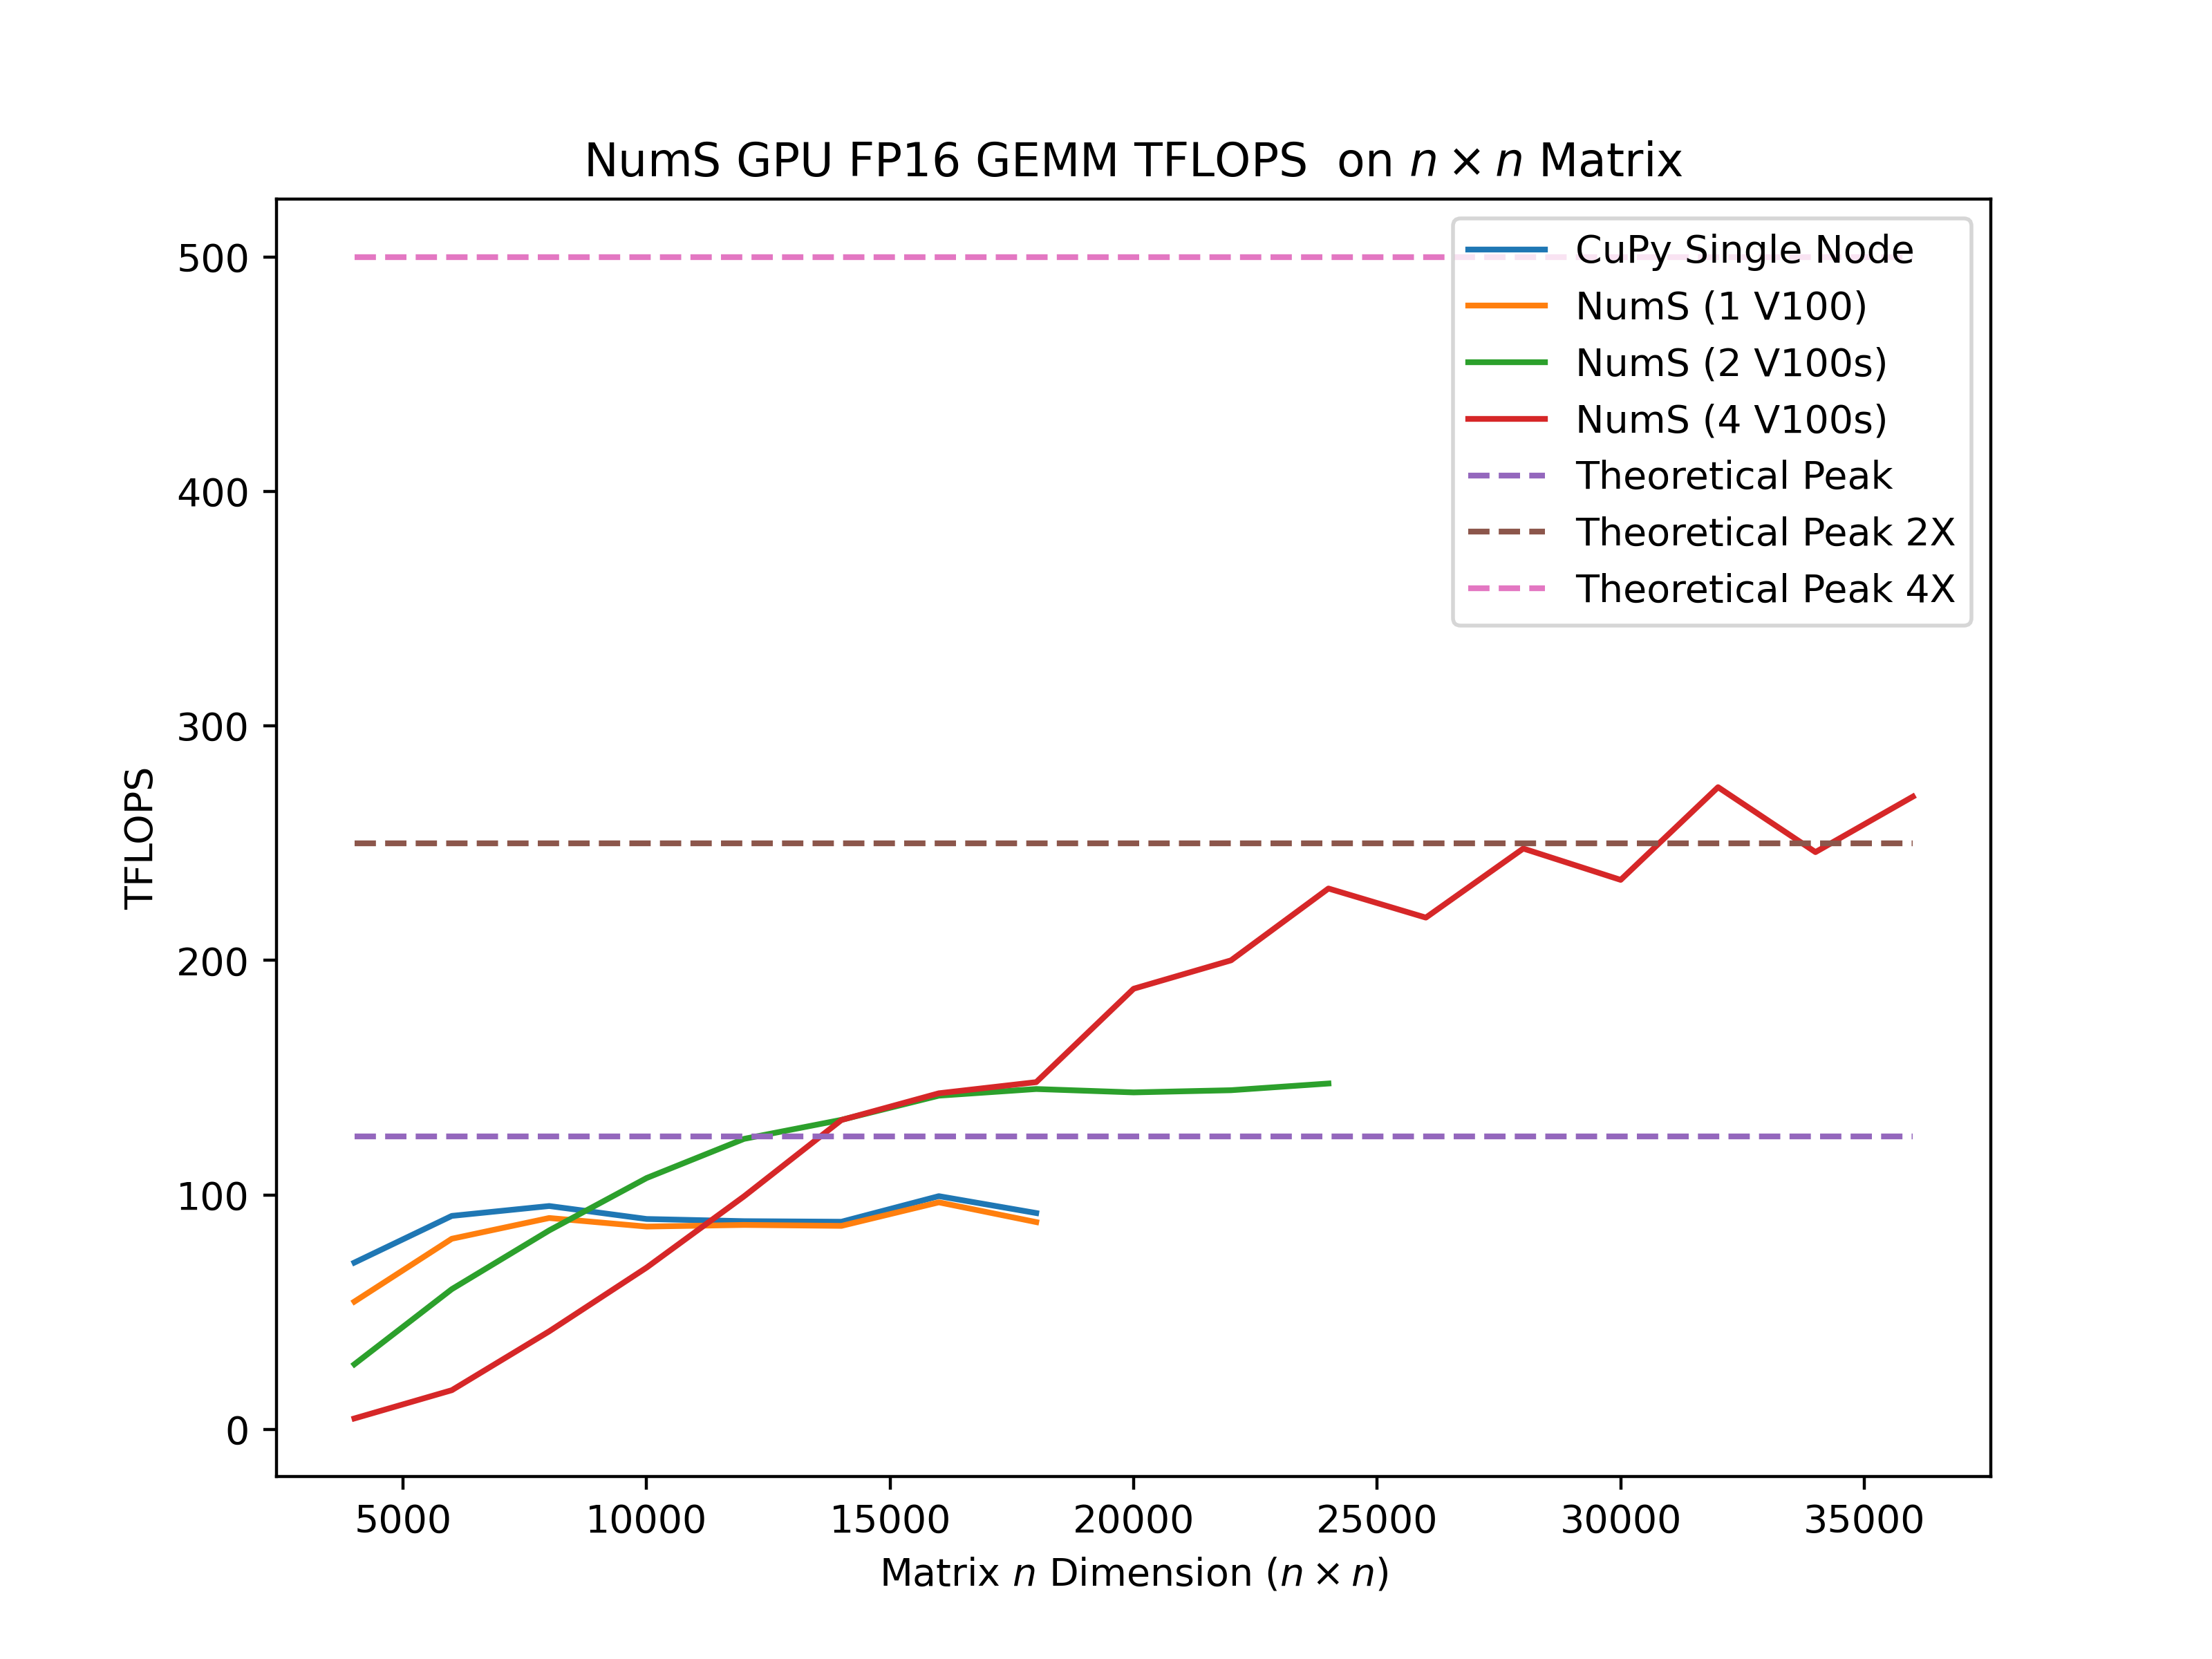
\includegraphics[width=5in]{figures/NumS_GPU_TFLOPS_FP16GEMM.png}}
	\caption{TeraFLOPs Half Precision (FP16) GEMM Benchmark}
	\label{fig:fp16gemm}
\end{figure}

\subsubsection{Elementwise Operations}
For elementwise operations, these are all handled by CuPy, as they are not a cuBLAS routine. Benchmarked are elementwise multiply of a $n$ size 1 dimensional array of double precision floating point numbers. Although the elementwise does not quite reach the theoretical peak, compared to just the normal CuPy implementation, it scales fairly well. Figure \ref{fig:elementwise} shows the performance, and the empirical peak is defined as the peak that CuPy can reach with a single GPU, which is 33.67 GFLOP/s. We see that this is able to maintain 85.60-97.77\% of the empirical peak that CuPy obtains when scaling to multiple GPUs.

\begin{figure}
	\centerline{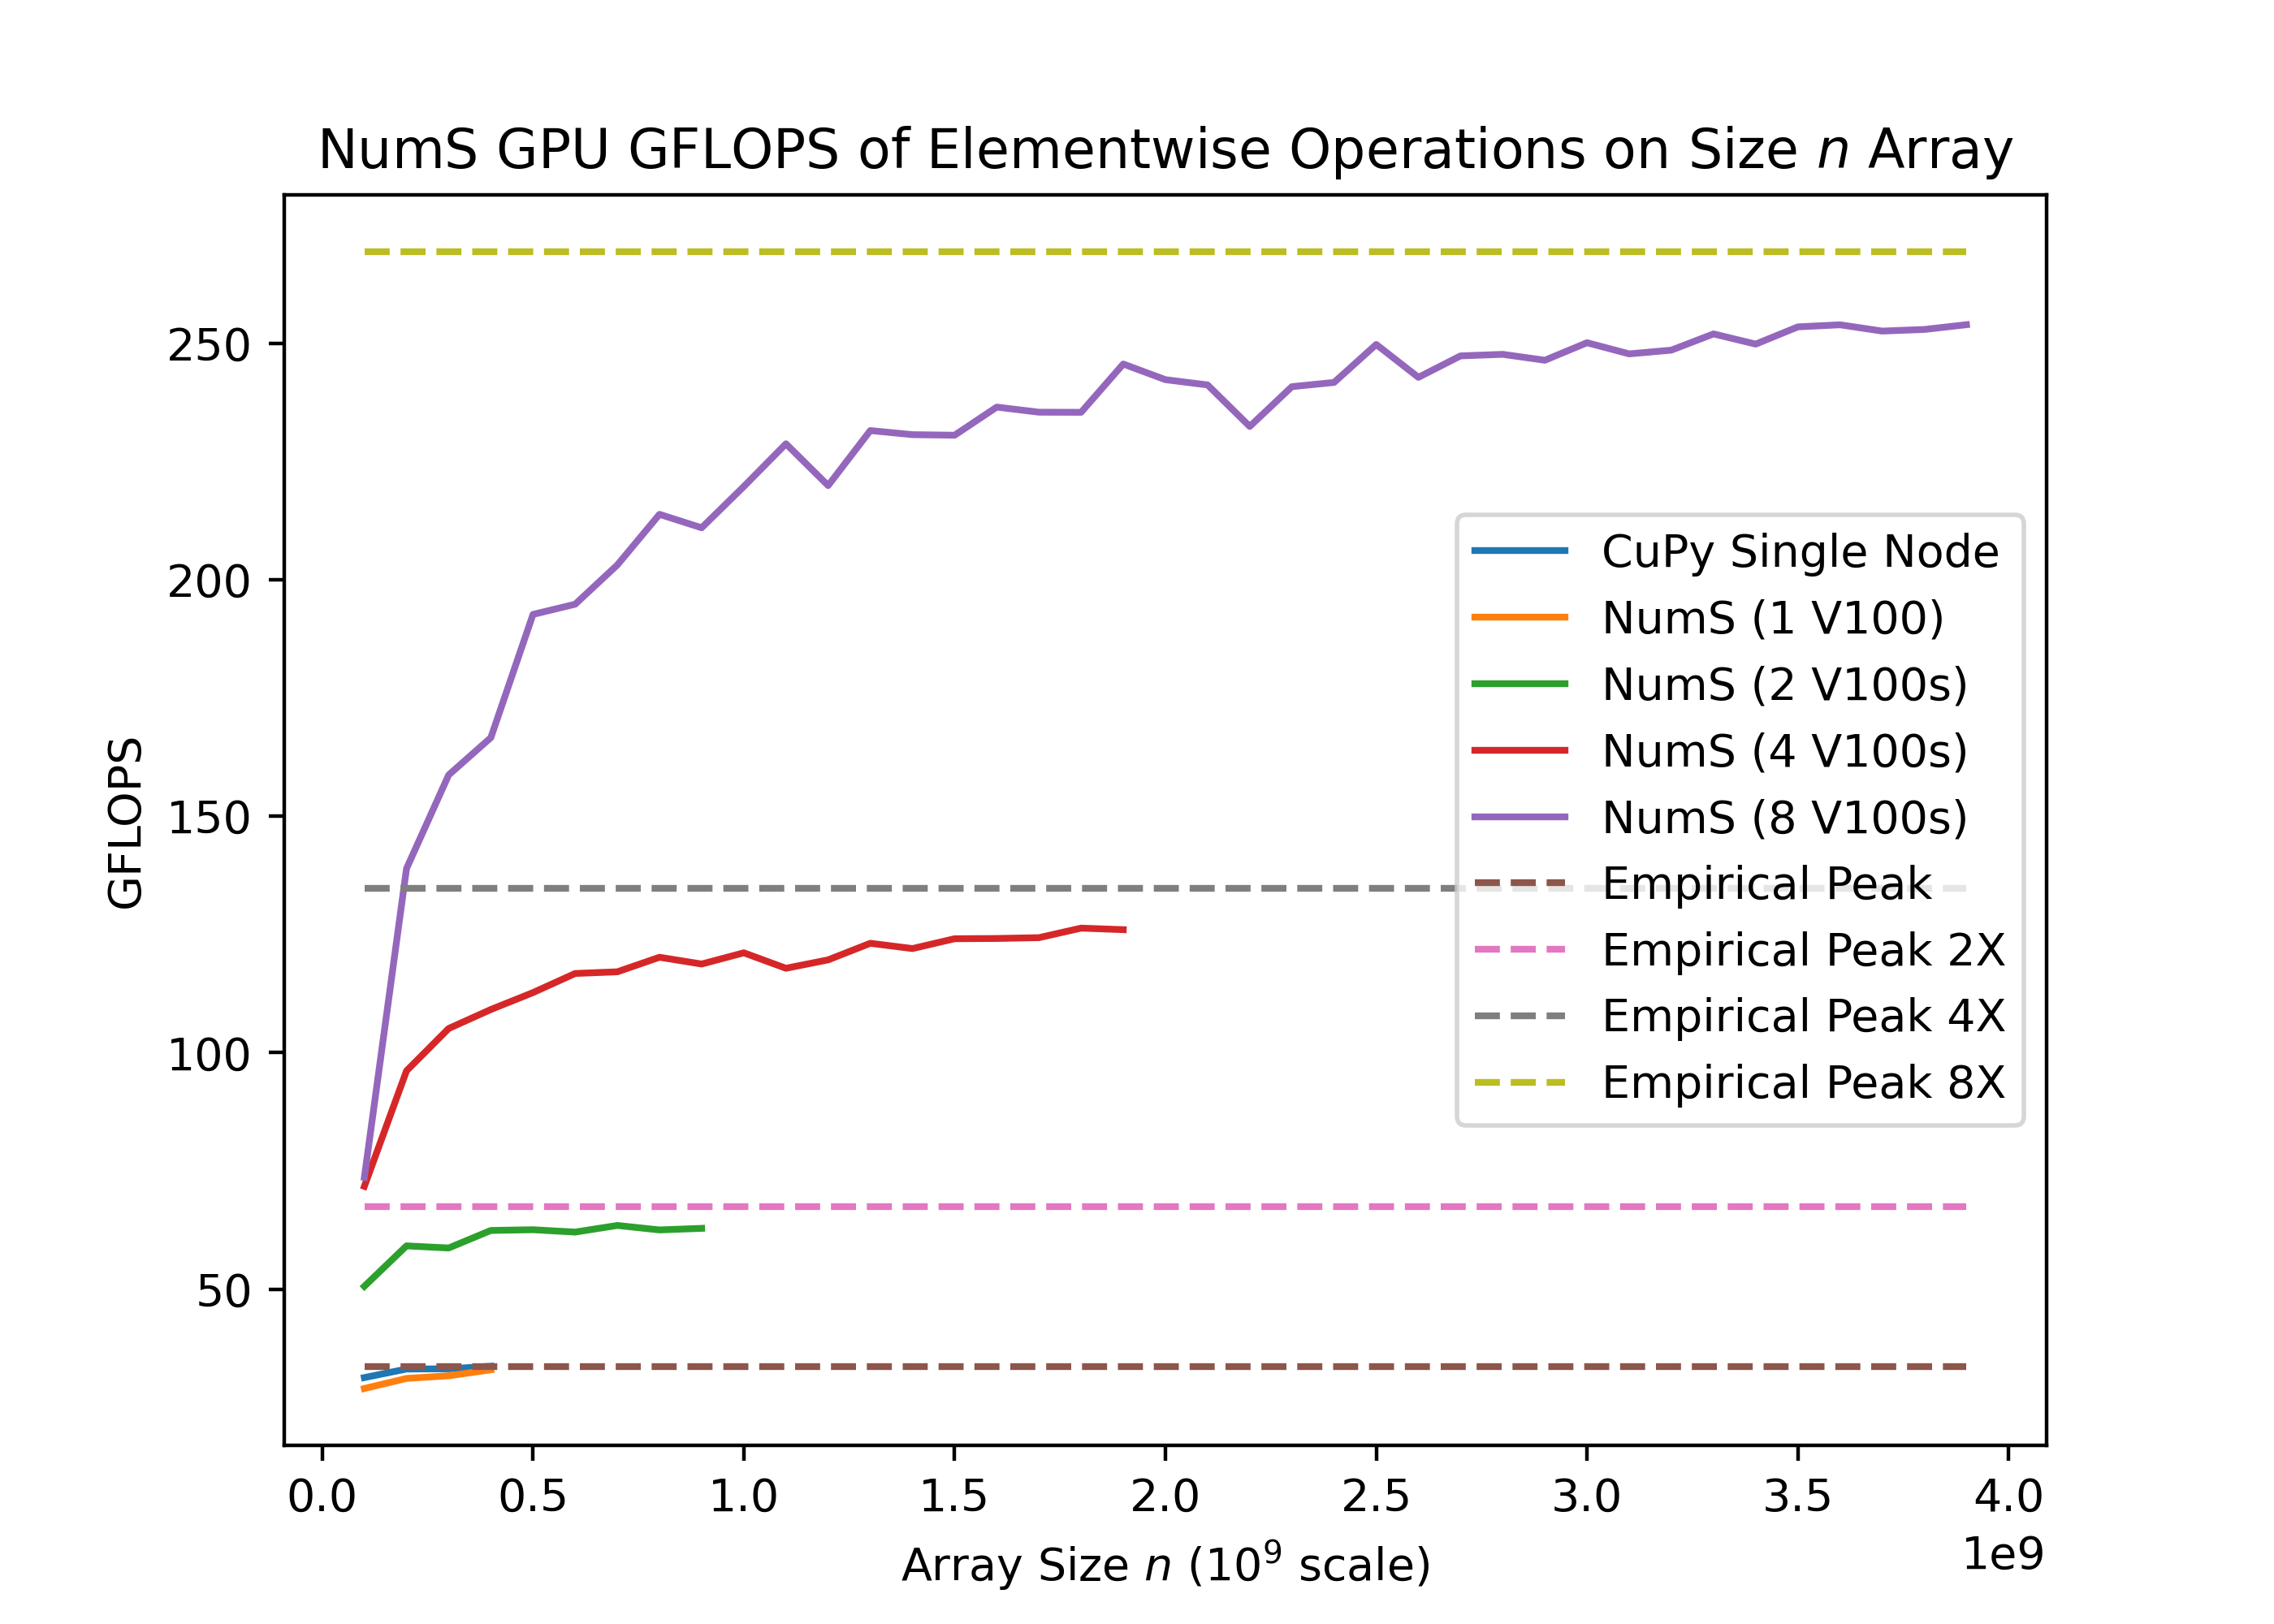
\includegraphics[width=5in]{figures/NumS_GPU_GFLOPS_elementwise.png}}
	\caption{GigaFLOPs Elementwise Benchmark}
	\label{fig:elementwise}
\end{figure}

\subsubsection{Logistic Regression}
NumS also provides distributed machine learning model training. For Logistic Regression performed on the HIGGS data set with a CPU Ray backend, NumS achieves on average 11.58 seconds of training time and 701.10 milliseconds of inference time. When compared against the GPU backend, NumS achieves on average 288.47 milliseconds of training time and 5.76 milliseconds of inference time. This is 40.14x faster for training and 121.72x faster for inference. Unfortunately, the CuPy API conflicts with NumS API with how vector shapes are handled, so we could not scale up the experiments to multiple GPUs when working with block partitioned arrays.

\subsubsection{Multi Layer Perceptron}
To further test how NumS works on machine learning model training, we built a simple multilayer perceptron (MLP). The MLP has two linear layers each followed by a rectified linear unit (ReLU) layer. The first layer has an output dimension of $100$ and the second layer has an output dimension of $200$. We generate a random dataset with 10 columns and and the model predicts one of two classes, making this a binary classification task that this MLP is solving for. Because the MLP had relatively small layers and the NumS API conflicted with CuPy API when scaling to larger inputs, we only tested against CPU on the Bridges-2 CPU.

Shown in Figure \ref{fig:mlp bench}, we see the performance benchmark of the MLP as the size of the data increases. We tested this with the two different backends offered in NumS (CPU and GPU), and added an additional comparison with the popular deep learning library Pytorch \cite{NEURIPS2019_9015}. We see that training time (Figure \ref{fig:mlp train}) certainly increases as the size of the data increases, but NumS does scale better than both a distributed CPU framework and Ray. In Figure \ref{fig:mlp inference}, we show the difference in inference time between CPU and GPU. We see here again a large magnitude of difference between the computational capabilities of the backend. While reduction operations are currently not implemented, we hope to extend the performance benefits offered by the GPU backend to a distributed setting.

\begin{figure}
	\centering
	\subfloat[\centering MLP Training Benchmark ]{{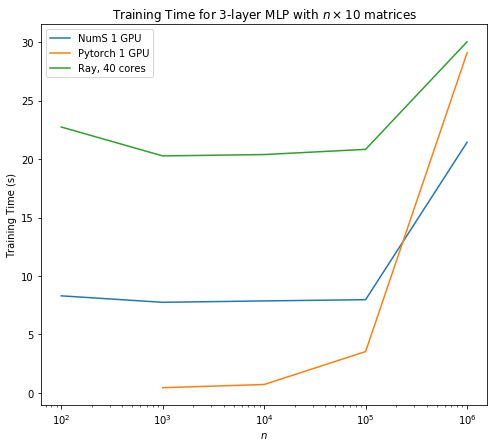
\includegraphics[width=8cm]{figures/tr.png} }
		\label{fig:mlp train}}

	\qquad
	\subfloat[\centering MLP Inference Benchmark]{{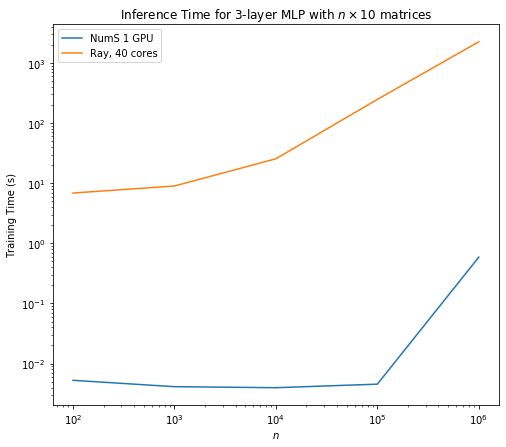
\includegraphics[width=8cm]{figures/inf.png} }
		\label{fig:mlp inference}}
	\caption{MLP Benchmarks using different backends. The training time is given on the $y$-axis and the size of the array is given on the $x$-axis.}
	\label{fig:mlp bench}
\end{figure}

\subsection{Energy and Cost Analysis}
Although the results and benchmarks sound promising, it's also important to consider if the compute costs are worth it.
An interesting way to look at the performance of GPUs is to compare it against cloud computing service rates such as AWS. \cite{aws} Here, we'll analyze the FLOPs per price ratio for double precision computations.

AWS's P3 instances use NVIDIA V100 GPUs that has rates scaling linearly with the number of GPUs. \verb|p3.2xlarge| takes \$3.06 per hour with on demand pricing for 1 GPU which equates to \$6.54 per PFLOP or 152.90 TFLOP/dollar.

$$\frac{\$3.06}{\textrm{hour}}\frac{1 \textrm{ hour}}{60 \textrm{s}}\frac{1 \textrm{s}}{0.0078\textrm{ PFLOP}} = \$6.54/\textrm{PFLOP}$$


Compared to a high performance CPU instance such as AWS's \verb|r5.16xlarge|, it costs \$4.032 for on demand pricing which equates to \$262.25 per hour or 3.964 TFLOP/dollar. The theoretical peak of \verb|r5.16xlarge|, which uses Intel(R) Xeon(R) Platinum 8259CL CPU, is 2.56 TFLOPs.

$$\frac{\$4.032}{\textrm{hour}}\frac{1 \textrm{ hour}}{60 \textrm{s}}\frac{1 \textrm{s}}{0.00256\textrm{ PFLOP}} = \$26.25/\textrm{PFLOP}$$

Theoretically, we see that there is a 4.01x difference in the price the user pays per PFLOP with On Demand Pricing on AWS. So for a high compute service in the cloud, a GPU can be much more cost saving if a program can utilize all of the resources provided by the GPU.

In HPC systems, we also care about the amount of power being consumed. Here, we'll compare two HPC compute nodes, Intel KNL on Cori Supercomputer and NVIDIA V100 on Bridges-2.

On NVIDIA V100, the TDP is 300 W. Since a watt can be also defined in joules/second, it takes 38.46 joules per TFLOP. \cite{v100}

$$\frac{300\textrm{ joules}}{\textrm{s}}\frac{\textrm{s}}{7.8 \textrm{ TFLOP}} = 38.46 \textrm{ joules/TFLOP}$$


On Intel KNL processor, the theoretical peak using all 68 cores is 3 TFLOPs. This equates to the processor using 71.67 joules per TFLOP. \cite{knl}

$$\frac{215\textrm{ joules}}{\textrm{s}}\frac{\textrm{s}}{3 \textrm{ TFLOP}} = 71.67 \textrm{ joules/TFLOP}$$

Thus, in theory it is 1.86x more energy saving to choose a GPU over a CPU in high compute tasks. We see that NumS with GPU support becomes a viable cost and energy saving option in dense linear algebra computations given the high percentage of theoretical peak obtained with DGEMM routines.

\section{Related Work}
For executing linear algebra on a multi-GPU systems, we see that it is still novel and in its early stages. For example, NVIDIA's cuBLAS Multi-GPU Extension is still in its Early Access phase. \cite{cublasmg} Dask also provides multi GPU support for array programming, but it's still in an experimental stage. \cite{dask-cuda}

\section{Conclusion}
Currently, distributed GPU computations are still a work in progress in the current state. Although we are able to achieve good scaling with non-communication algorithms, we find the performance on communication algorithms a challenge, such as matrix multiply. The limitation of scalability is not as easy to pinpoint as it could come from NVIDIA's NCCL library performance or the design of NumS.

For Ray, debugging performance, especially on a HPC environment can be hard to pinpoint. Python processes become wrapped under Ray processes and it becomes hard to profile CUDA API calls through profilers like NVIDIA NSight Systems. Thus, it was much easier to figure out performance bugs with NCCL as it profiles everything including memory transfers, NCCL, cuBLAS, and CUDA API calls. Ray also has it's own profilers, but it is not as verbose as NSight.

A limitation of GPUs is memory. GPU has its own memory which is not user upgradable, meaning that there is hard limit on memory constraints. As such, if memory is a constraint to the user, such as operating on terabytes of data, then using CPU with a configurable expandable memory may be preferable oppopsed to the gigabytes of memory GPUs can scale to.

Adding GPU support also allows users to run hardware agnostic code when using NumS. For example, a user can train on cheap distributed instances using CPU and Ray backend, and for inference, where performance is often crucial, they can switch to a GPU backend. As mentioned by Borrill, computational scientists are limited by what their HPC vendor can supply, and a change in HPC Architecture such as many core CPU to GPU means that users will have to translate their code to other parallel primitives. \cite{borrill} In this example, it could probably be converting from Intel Intrinsics, OpenMP, and MPI to CUDA. With NumS, users can just change the backend with a single line of code and easily run from a CPU to GPU environment.

\section{Future Work}
For future work, we wish to explore how to extend scalability to even more GPUs and to inter-node systems. The main challenge in properly designing such a system is efficiently scheduling within intra-node and between inter-node. We also only focused on HPC systems with the use of Bridges-2. But other work could be done to also try to deploy this on AWS cloud services, as they also provide V100 instances with P3 instances. There are many limitations from Ray that prevent it from working in an HPC environment such as being able to run smoothly on a Slurm environment and tight network security on ports. There are workarounds available, but due to the fast growing pace of the Ray community and it's focus on the cloud, it becomes outdated quickly by newer versions of Ray.

We could also try to improve the collective communication calls for certain algorithms to utilize \verb|BCast|, \verb|AllReduce|, \verb|Reduce|, and \verb|AllGather|. Lastly, tuning the block sizes of NumS BlockArrays is also something we haven't explored, and it would be beneficial to do along with a strong analysis and optimization of communication over NVLink.

\section{Contributions}
The benchmarks collected in this report are publicly available in this repository. \cite{benchmarks} The draft of the GPU implementation is also available here. \cite{nums-pr}

\bibliographystyle{ieeetr}
\bibliography{references}

\end{document}
